\documentclass{beamer}
\usetheme{Warsaw}
\setbeamertemplate{caption}[numbered]
\setbeamertemplate{navigation symbols}{}%remove navigation symbols

\usepackage{polski}
\usepackage[utf8]{inputenc}
\usepackage{array}
\usepackage{hyperref}

\title{Optymalizacja struktury sieci drogowej}
\author{Michał Siatkowski} 
\institute{Promotor: dr hab. inż. Aneta Poniszewska - Marańda \\
		Kopromotor: mgr inż. Łukasz Chomątek \\
		\vspace*{20px}
		Politechnika Łódzka}
\date{Łódź, FTIMS, Informatyka 2014/2015}

\begin{document}

\maketitle

\section{Wstep}
\subsection{Problematyka i zakres pracy}
\begin{frame}{Problematyka i zakres pracy} 

Niniejsza praca obejmuje zagadnienia z zakresu inżynierii oprogramowania i sztucznej inteligencji. Głównym jej celem jest stworzenie aplikacji optymalizującej strukturę sieci drogowej.

\end{frame}

\subsection{Cele pracy}
\begin{frame}{Cele pracy} 

Celami pracy są:
\begin{enumerate}

\item Zdefiniowanie problematyki optymalizacji struktury sieci drogowej.
\item Stworzenie aplikacji optymalizującej tę strukturę.
\item Analiza i ocena efektywności zastosowanych rozwiązań.

\end{enumerate}

\end{frame}

\subsection{Metoda badawcza}
\begin{frame}{Metoda badawcza} 
\newtheorem{mydef0}{Prototypowanie}
\begin{mydef0}
jest to proces budowy modelu matematycznego i obserwacja czy jego zachowanie może pomóc inżynierom w odkryciu ukrytych wad ich projektu. Z założenia prototypy nie wchodzą w skład ostatecznego systemu.
\end{mydef0}
\end{frame}

\subsection{Przeglad literatury w dziedzinie}
\begin{frame}{Przeglad literatury w dziedzinie} 

\begin{enumerate}

\item {
Wataru Nanya, Hiroshi Kitada, Azusa Hara, Yukiko Wakita, Tatsuhiro Tamaki, and Eisuke Kita\\
\emph{Road Network Optimization for Increasing Traffic Flow}. International Conference on Simulation Technology, JSST 2013.}

\end{enumerate}
\end{frame}


\section{Optymalizacja struktury sieci drogowej}
\subsection{Podstawowe definicje}
\begin{frame}{Podstawowe definicje} 

\newtheorem{mydef1}{Sieć drogowa}
\begin{mydef1}
	\begin{figure}[h!]
	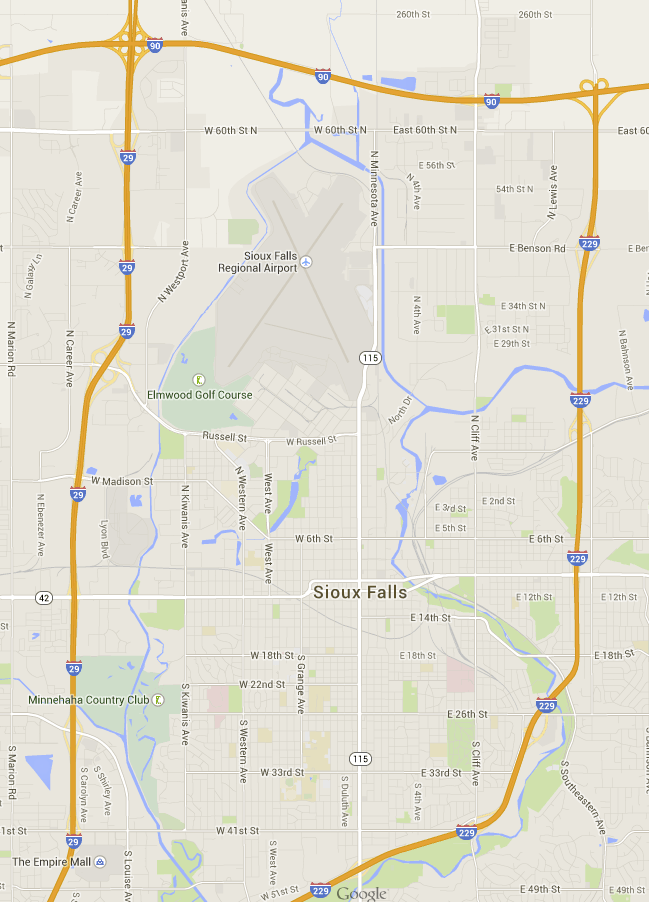
\includegraphics[width=0.30\textwidth]{img/siec}
	\caption{Fragment sieci drogowej w Sioux Falls, Południowa Dakota.} 
	\end{figure}
\end{mydef1}

\end{frame}

\begin{frame}{Podstawowe definicje} 

\newtheorem{mydef2}{Sieć drogowa w postaci grafu}
\begin{mydef2}
	\begin{figure}[h!]
	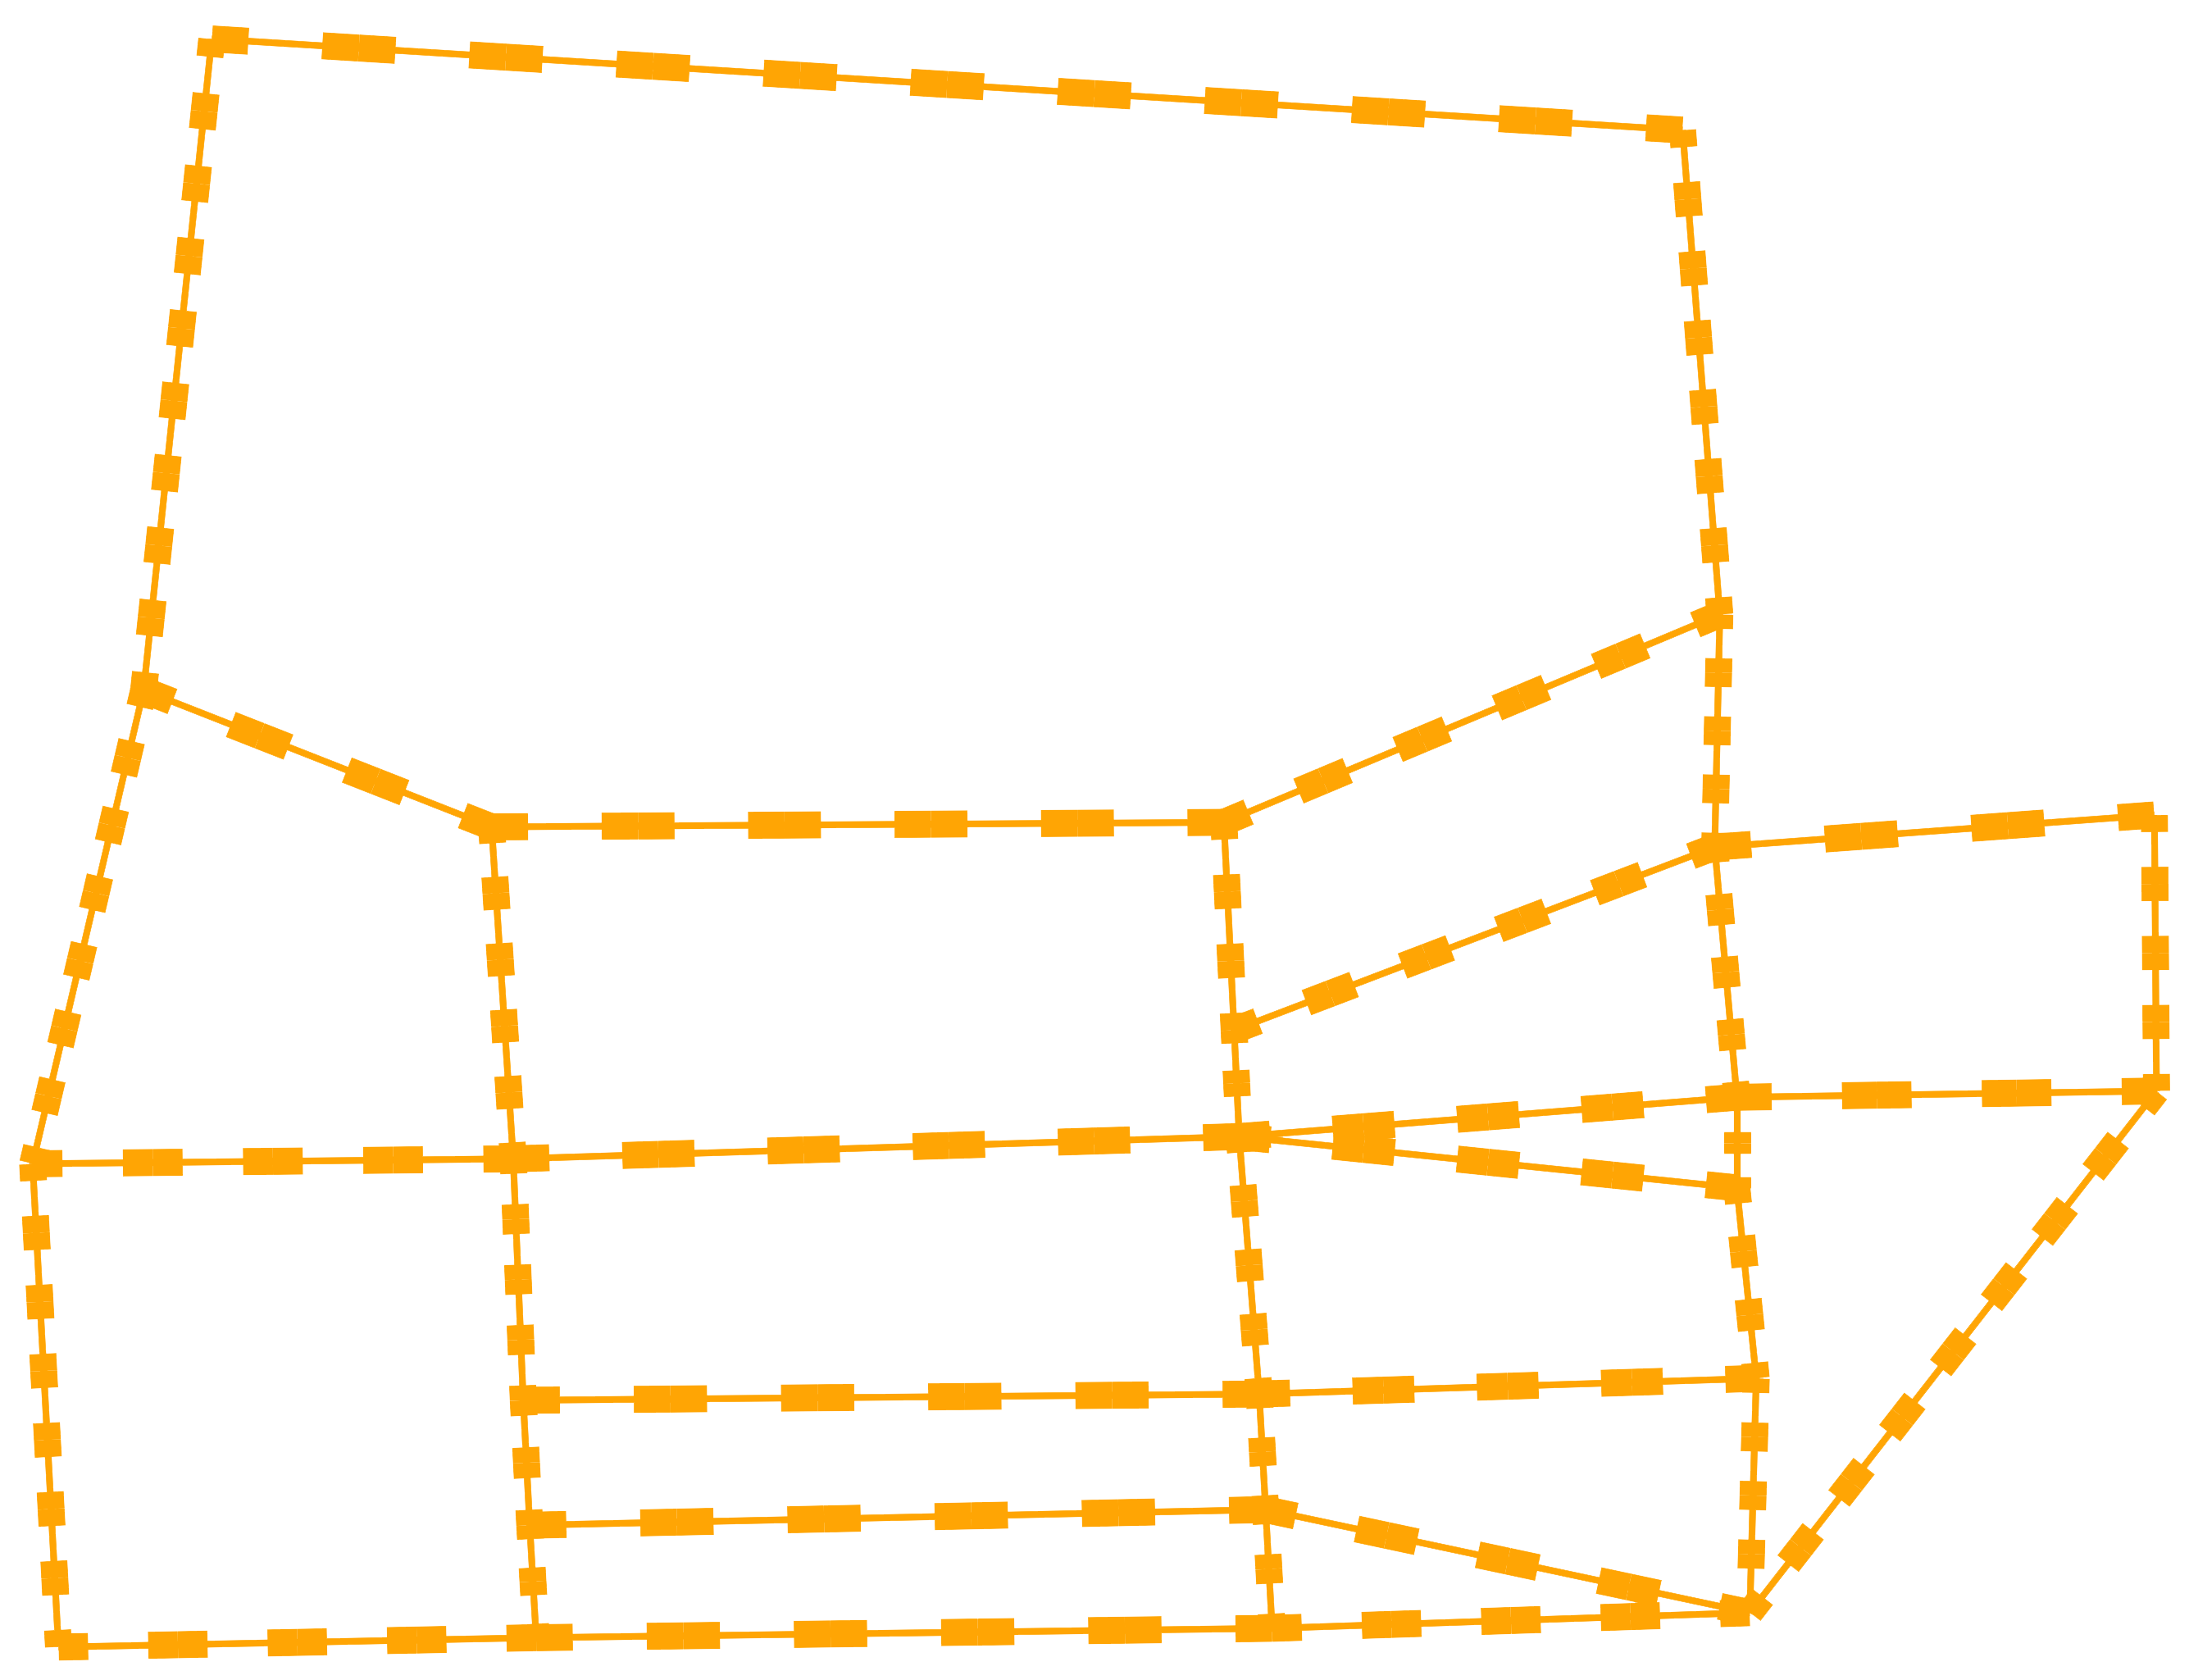
\includegraphics[width=0.55\textwidth]{img/graf}
	\caption{Siec drogowa miasta Sioux Falls w postaci grafu.} 
	\end{figure}
\end{mydef2}

\end{frame}

\begin{frame}{Podstawowe definicje} 
	\begin{figure}[h!]
	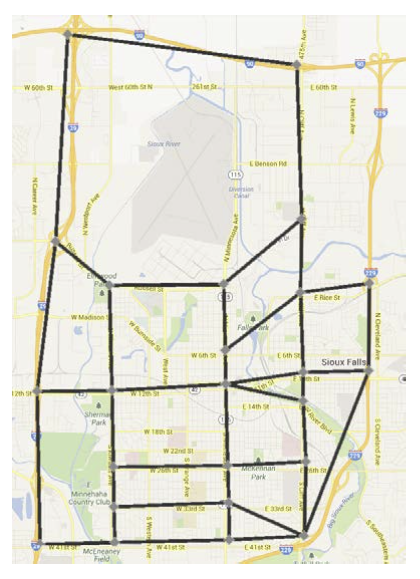
\includegraphics[width=0.38\textwidth]{img/dopasowanie}
	\caption{Graf z dopasowaną geometrią \cite{siux}.}
	\end{figure}
\end{frame}


\subsection{Paradoks Braessa }
\begin{frame}{Paradoks Braessa\cite{braess}}

\centering
\begin{minipage}{.48\textwidth}
\begin{figure}[h!]
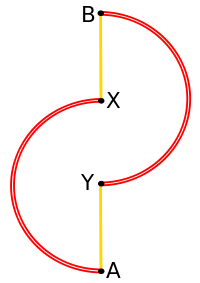
\includegraphics[width=0.7\textwidth]{img/braess1}
\caption{Wyjściowy układ drogowy}
\end{figure}
\end{minipage}\hfill
\begin{minipage}{.48\textwidth}

Autostrady:\\
AX, $t_{AX}(p) =  50 + p$ min\\
BY, $t_{YB}(p) =  50 + p$ min\\

Drogi lokalne:\\
BX, $t_{XB}(p) =  10p$ min\\
AY, $t_{AY}(p) =  10p$ min\\
\\
Aut jest 6000 i wszystkie mają za zadanie przejechać trasę z A do B.

\end{minipage}\hfill

\end{frame}


\begin{frame}{Równowaga Nasha\cite{braess}} 

Równowaga Nasha to taka sytuacja, w której każdy z samochodów spowoduje wydłużenie swojego czasu jazdy, zmieniając decyzję co do wyboru trasy przy niezmienionych decyzjach pozostałych aut.
\newline\newline
Jeśli p i q to liczby aut w tysiącach pokonujących odpowiednio trasy AXB i AYB, otrzymujmy równania:

\begin{center}
$p+q = 6 $\\
$t_{AX}(p)+t_{BX}(p) = t_{AY}(q) + t_{BY}(q)$\\
$50+p+10p = 10q+50+q$
\end{center}
rozwiązaniem jest $p=q=3$.\\
Przy tej gęstości ruchu pokonanie obu dostępnych tras zabiera $50+3+30=83$ minuty.
\end{frame}

\begin{frame}{Uzupełniony układ drogowy \cite{braess}} 

\centering
\begin{minipage}{.48\textwidth}
\begin{figure}[h!]
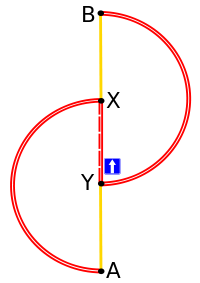
\includegraphics[width=0.7\textwidth]{img/braess2}
\caption{Uzupełniony układ drogowy}
\end{figure}
\end{minipage}\hfill
\begin{minipage}{.48\textwidth}
Do wyjściowego układu drogowego dodana zostaje autostrada:\\

YX, $t_{YX}(p) =  10 + p$ min\\

Aut jest nadal 6000 i wszystkie mają za zadanie przejechać trasę z A do B.

\end{minipage}\hfill
\end{frame}

\begin{frame}{Równowaga Nasha dla uzupełnionego układu\cite{braess}} 

Jeśli p, q i r to liczby aut w tysiącach pokonujących odpowiednio trasy AXB, AYB i AYXB, otrzymujmy równania:

\begin{center}
$p+q+r = 6 $\\
$t_{AX}(p)+t_{BX}(p+r) = t_{AY}(q+r) + t_{BY}(q) = t_{AY}(q+r)+t_{YX}(r)+t_{XB}(p+r)$
\newline\\
$50+p+10(p+r) = 10(q+r)+50+q = 10(q+r)+ 10 + r + 10(p+r)$
\end{center}
rozwiązaniem jest $p=q=r=2$.\\
Czas przejazdu każdej z tych dróg wynosi wówczas $50+2+10(2+2)=92$ minuty.
\end{frame}


\subsection{Słabe punkty istniejacych rozwiazań}
\begin{frame}{Słabe punkty istniejacych rozwiazań} 

Paradoks Braessa został sformułowany w roku 1970,
a od roku 1996 zaczęły pojawiać się prace negujące lub podważające paradoks\cite{newinsights}.
Wiele miast jednak brało i bierze pod uwagę paradoks Braessa podczas projektowania swojej przestrzeni:

\begin{itemize}
\item Korea, Seul, likwidacja m.in. estakad Cheonggyecheon,
\item Niemcy, Stuttgart, likwidacja dróg zbudowanych w latach 60,
\item USA, Nowy Jork, czasowe zamknięcie ulicy 42,
\item USA, Winnipeg.\cite{urban}
\end{itemize}  

\end{frame}


\section{Technologie i metody użyte}


\subsection{Symulator transportu}
\begin{frame}{Symulator transportu} 

	\begin{figure}[h!]
	
\includegraphics[width=0.30\textwidth]{img/matsim}
	\caption{Logo symulatora transportu MATSim \cite{matsim}} 
	\end{figure}

\end{frame}

\subsection{Przestrzeń poszukiwań}
\begin{frame}{Przestrzeń poszukiwań} 

Najlepszego rozwiązania będę poszukiwał wykorzystując algorytm genetyczny.

\end{frame}


\subsection{Technologie i metodologie programistyczne}
\begin{frame}{Technologie i metodologie programistyczne} 

\centering
\begin{minipage}[b]{.48\textwidth}

\begin{figure}

\includegraphics[width=0.7\textwidth]{img/java}
\caption{Logo języka Java\cite{java}}
\end{figure}
\begin{figure}

\includegraphics[width=0.7\textwidth]{img/eclipse}
\caption{Logo aplikacji IDE Eclipse\cite{eclipse}}
\end{figure}

\end{minipage}\hfill
\begin{minipage}[b]{.48\textwidth}

\begin{figure}

\includegraphics[width=0.7\textwidth]{img/py}
\caption{Logo języka Python\cite{python}}
\end{figure}
\begin{figure}

\includegraphics[width=0.55\textwidth]{img/pydev}
\caption{Logo rozszerzenia PyDev\cite{pydev}}
\end{figure}

\end{minipage}\hfill
\end{frame}

\section{Aplikacja knoWledge}

\subsection{Analiza wymagań}
\begin{frame}{Analiza wymagań} 
\begin{itemize}
\item{Użytkownik może korzystać z konta "tymczasowego" dla niezalogowanej sesji}
\item{Użytkownik może się zarejestrować na portalu}
\item{Użytkownik może się zalogować na portalu}
\item{Użytkownik może komentować treść portalu, oceniać ją, co wpływa na treść wyświetlaną dla
	danego użytkownika}
\item{Użytkownik może dodawać do znajomych innych użytkowników portalu}	
\item{Użytkownik może filtrować treść portalu względem gustów innych użytkowników}
\end{itemize}
\end{frame}


\subsection{Projekt bazy danych}
\begin{frame}{Projekt bazy danych}
Informacje o użytkownikach są przechowywane w bazie danych
\begin{itemize}
\item{Tabela użytkowników}
\item{Tabela komentarzy}
\item{Tabela artykułów}
\item{Tabela ocen}
\end{itemize}
\end{frame}


\subsection{Implementacja: punkty kluczowe}
\begin{frame}{Implementacja: punkty kluczowe} 
\newtheorem{mydef4}{Filtrowanie uwspólnione}
\begin{mydef4}

Każdy użytkownik jest traktowany jako n-wymiarowy wektor pozycji dostępnych na portalu. Każdy element wektora jest oceną danej pozycji, np. w skali 0 (brak oceny) - 10. Dla przeciętnego użytkownika wektor ten będzie wektorem rzadkim, tzn. będzie występować dużo wartości zerowych. Algorytm, generuje rekomendację w oparciu o grupę użytkowników najbardziej podobnych do rozważanego użytkownika porównując miarę podobieństwa przy użyciu wzoru na cosinusową miarę podobieństwa wektorów:$ ^{[1]} $ \\ 

\begin{center}
$ podobieństwo(\overrightarrow{A},\overrightarrow{B}) = cos(\overrightarrow{A},\overrightarrow{B}) =  \frac{a_1 b_1 + a_2 b_2 + \ldots + a_n b_n }{ \sqrt{a_1^2 + a_2^2 + \ldots + a_n^2 }  \cdot \sqrt{b_1^2 + b_2^2 + \ldots + b_n^2 }} $
\end{center}
\end{mydef4}
\end{frame}


\subsection{Wdrożenie}
\begin{frame}{Wdrożenie} 

Przy pomocy Media Wiki API treść haseł Wikipedii będzie wyświetlana jako główna część strony.
Oprócz tego z treści artykułu zostaną wyodrębnione jego kategorie oraz artykuły, do których zawiera bezpośrednie połączenia (linki). Na podstawie tych danych stworzona zostanie siatka powiązań pomiędzy hasłami a oceniając dany artykuł będziemy modyfikować wielkości odpowiadających elementów wektora ocen.

\end{frame}


\subsection{Przewidywane problemy}
\begin{frame}{Przewidywane problemy} 
\newtheorem{mydef3}{Zimny start (Cold start)}
\begin{mydef3}
Problem typowy dla systemów rekomendacyjnych. Przejawia się brakiem treści do analizy dla systemu, a co za tym idzie, niemożność przedstawienia wyników. $ ^{[1]} $
\end{mydef3}

Rozwiązanie:\\
Integracja portalu z Facebookiem, korzystanie z profilu danego użytkownika.

\end{frame}


\section{Podsumowanie}

\subsection{Dyskusja wyników}
\begin{frame}{Dyskusja wyników} 

Celem pracy jest uzyskanie działającej aplikacji sieciowej, dynamicznie pobierającej treść z portalu Wikipedia.org oraz działający system oceny tej treści.\\
Drugim celem jest zbadanie efektywności systemu rekomendacyjnego przy pomocy pierwiastkowego błędu średniokwadratowego.  $ ^{[1]} $ \\

\begin{center}$ RMSE = \sqrt{ \frac{1}{|\tau|} \displaystyle\sum\limits_{u,i \in  \tau } (\hat{r}_{ui}- r_{ui})^2}$ \end{center} 

Błąd obliczany jest dla przygotowanych wcześniej, pewnych, zestawów danych.

\end{frame}


\subsection{Perspektywy dalszych badań w dziedzinie}
\begin{frame}{Perspektywy dalszych badań w dziedzinie} 

\begin{itemize}
\item Wdrożenie hybrydowego systemu rekomendowania treści; uwspólnionego z kontekstowym.
\item Zastosowanie innych funkcji matematycznych do wybierania treści podobnych
\item Porównanie i ocena wybranych rozwiązań
\end{itemize}

\end{frame}


\section{Bibliografia}
\begin{frame}[allowframebreaks]{Bibliografia}
\begin{thebibliography}{10}

\bibitem{investigation} 
	Leslie Arthur Keith Bloy, 
	\newblock \textit{An investigation into Braess’ paradox}, 02/2007

\bibitem{newinsights}
	Rric Pas and Shari Principio
	\newblock \textit{Braess’ paradox: Some new insights}, April 1996

\bibitem{conference} 
	Wataru Nanya, Hiroshi Kitada, Azusa Hara, Yukiko Wakita, Tatsuhiro Tamaki, and Eisuke Kita
	\newblock \textit{Road Network Optimization for Increasing Traffic Flow}
	\newblock Conference on Simulation Technology, JSST 2013.

\bibitem{reducingtheeffects}
	Ana L. C. Bazzan and Franziska Klügl
	\newblock \textit{Reducing the Effects of the Braess Paradox with Information Manipulation}


\framebreak

\bibitem{matsim} 
	\url{http://matsim.org}	

\bibitem{jgap}
	\url{http://jgap.sourceforge.net}

\bibitem{java} 
	\url{http://www.java.com/pl/}

\bibitem{eclipse} 
	\url{https://eclipse.org}
				
\bibitem{python} 
	\url{http://pl.python.org}
	
\bibitem{pydev} 
	\url{http://pydev.org}

\framebreak

\bibitem{matsim-userg}
	M. Rieser, C. Dobler, T. Dubernet, D. Grether, A. Horni, G. Lammel, R. Waraich, M. Zilske, Kay W. Axhausen, Kai Nagel
	\newblock \textit{MATSim User Guide}
	\newblock updated September 12, 2014

\bibitem{siux}
	A. Chakirov
	\newblock \textit{Enriched Sioux Falls Scenario with Dynamic Demand}
	\newblock MATSim User Meeting, Zurich/Singapore, June 2013.
	
\bibitem{braess}
	\url{http://pl.wikipedia.org/wiki/Paradoks_Braessa}
	
\bibitem{urban}
	\url{http://urbnews.pl/paradoks-braessa/}
		
\end{thebibliography}
\end{frame}

\end{document}